\documentclass[12pt]{article}
\usepackage[utf8]{inputenc}
\usepackage[a4paper]{geometry}
\usepackage{graphicx}
\usepackage{amsmath}

\title{COMP6212 Assignment 2}
\author{James Robinson}

\begin{document}

	\maketitle

	\section{Question 1}

	\subsection{Part a}

	Figure~\ref{fig:p1} shows the trader's profit as a function of the asset price at the time the options mature, assuming both options have a cost of 0. If the asset price at maturity is less than 40, the trader exercises their put option, making a profit of $40 - S(T)$. If the asset price at maturity is greater than 45, they exercise their call option and make a profit of $S(T) - 45$.

	\begin{figure}[h]
		\centering
		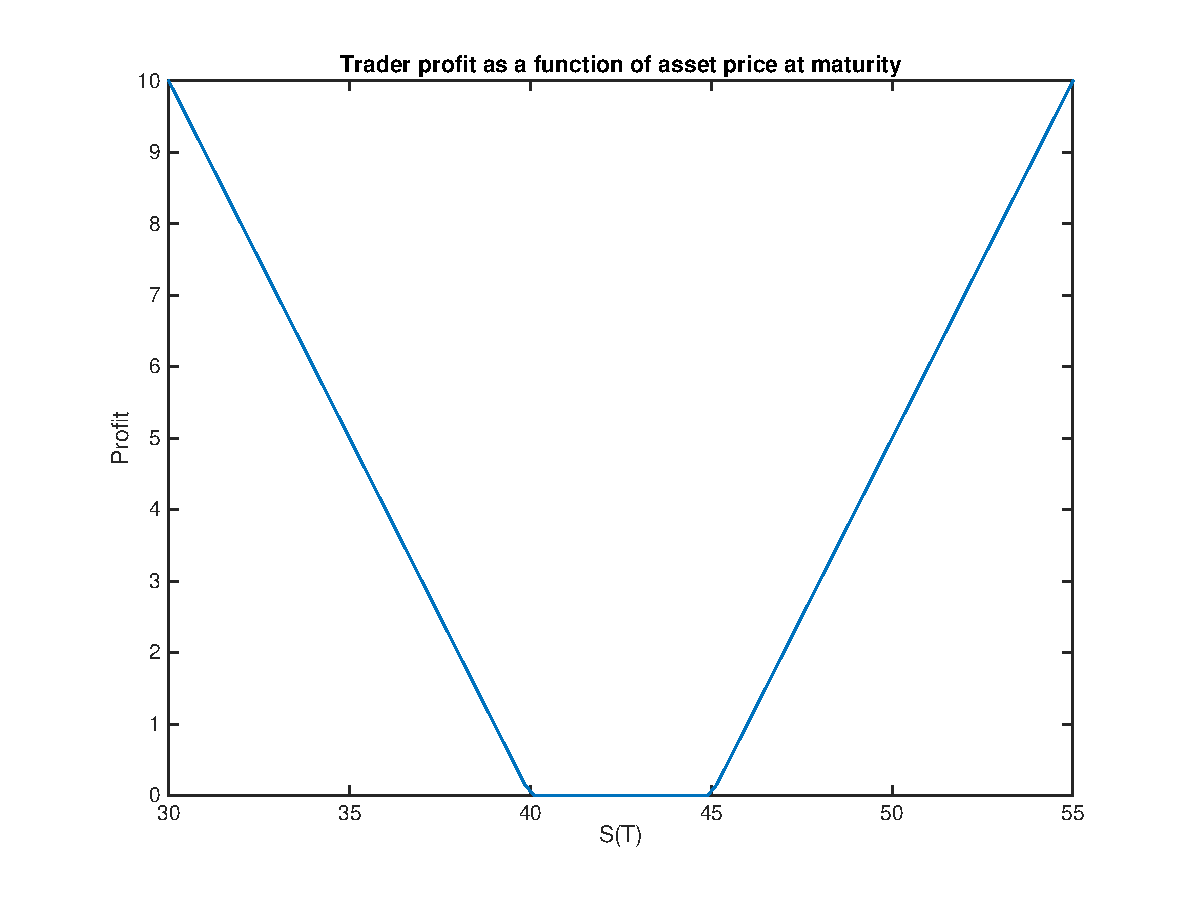
\includegraphics[width=0.5\linewidth]{figures/p1.eps}
		\caption{Trader profit as a function of asset price at option maturity}
		\label{fig:p1}
	\end{figure}

	\subsection{Part b}

	\subsubsection{Part 1}

	$$\mathcal{N}'(x) = \frac{1}{\sqrt{2\pi}} \exp\left(-\frac{1}{2} x^2\right)$$

	\subsubsection{Part 2}

	$$S\mathcal{N}'(d_1) = \frac{S}{\sqrt{2\pi}} \exp\left(-\frac{1}{2} d_1^2\right)$$

	$$= \frac{S}{\sqrt{2\pi}} \exp\left(-\frac{1}{2} \left(d_2 + \sigma\sqrt{T - t}\right)^2\right)$$

	$$= \frac{S}{\sqrt{2\pi}} \exp\left(-\frac{1}{2} \left(d_2^2 + 2d_2\sigma\sqrt{T - t} + \sigma^2(T - t)\right)\right)$$

	$$= \frac{S}{\sqrt{2\pi}} \exp\left(-\frac{1}{2}d_2^2 - d_2\sigma\sqrt{T - t} - \frac{1}{2}\sigma^2(T - t)\right)$$

	I don't know where to go from here.

	\subsubsection{Part 3}

	$$\frac{\partial d_1}{\partial S} = \frac{\partial d_2}{\partial S} = \frac{1}{\sigma S \sqrt{T - t}}$$

	\subsubsection{Part 4 and 5}

	???

	\section{Question 2}

	The Black-Scholes model underestimated the values of a number of options, most notably the put option with strike price 2925 and the call option with strike price 3325. The prices estimated by the Black-Scholes model in these cases (0 for each at every point in time) make intuitive sense - in the former case the strike price is always below the asset price, and in the latter, the strike price is always above, such that exercising either contract is pointless. It is unclear to me why the actual prices of these two options are so high.

	For the options with sensible strike prices, the Black-Scholes model was able to accurately predict the actual option prices.

	\newgeometry{top = 1cm, left = 1cm, right = 1cm}
	\begin{figure}
		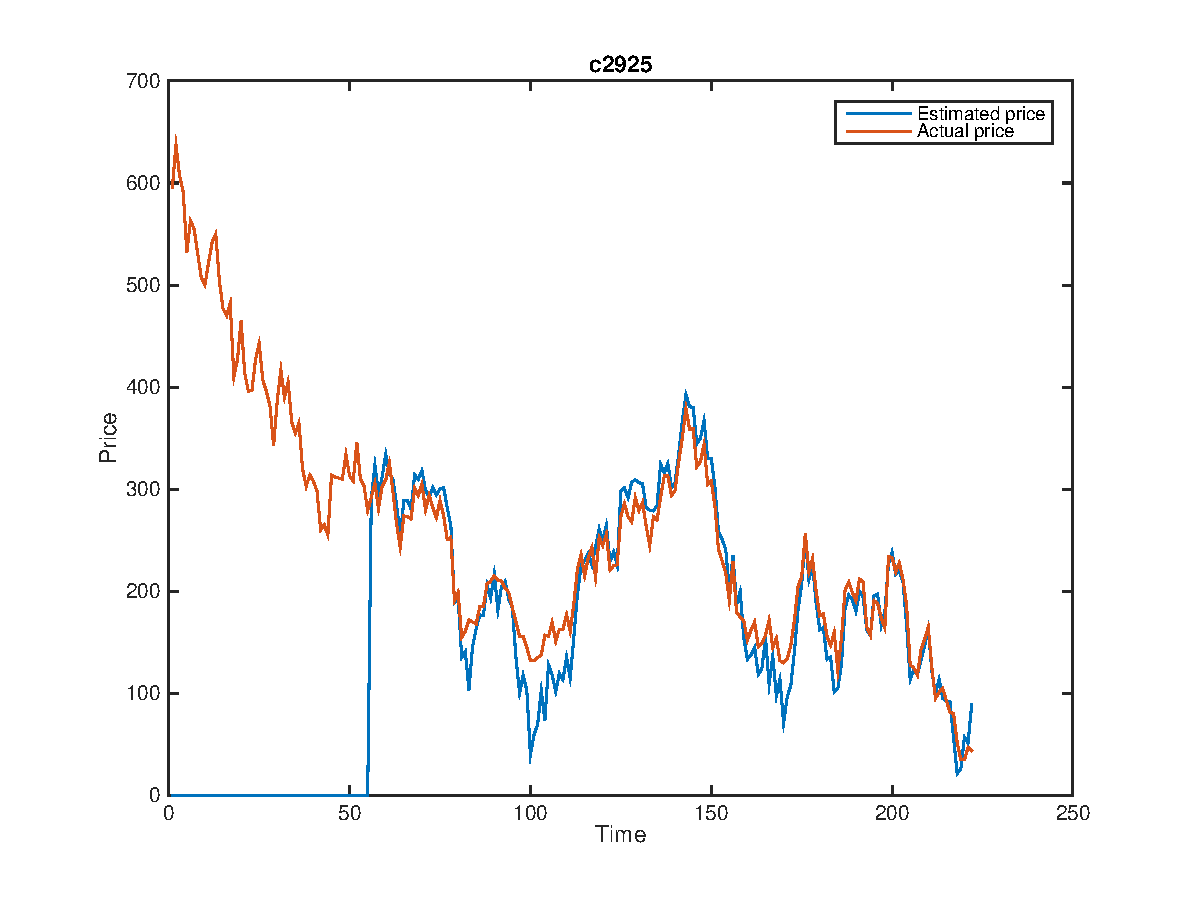
\includegraphics[width=0.32\linewidth]{figures/p2/1.eps}
		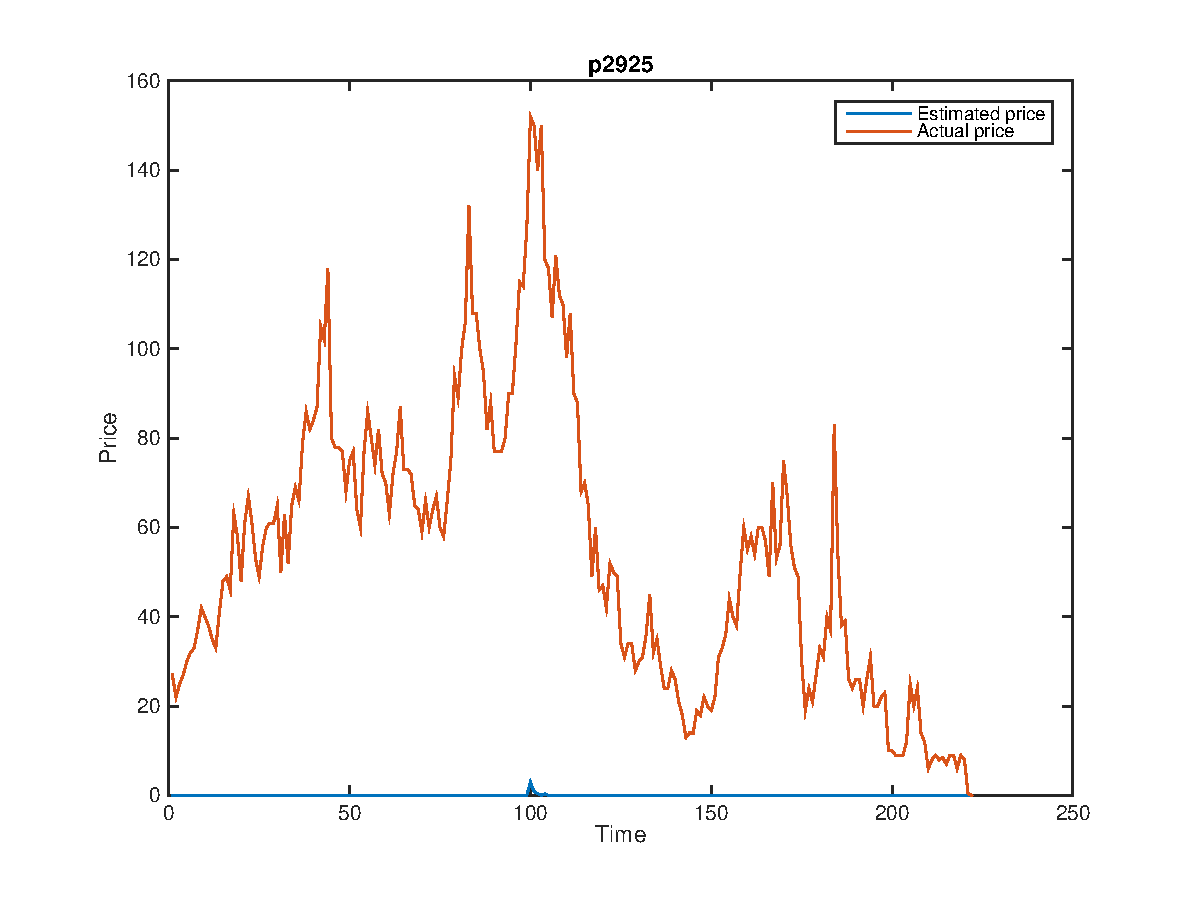
\includegraphics[width=0.32\linewidth]{figures/p2/2.eps}
		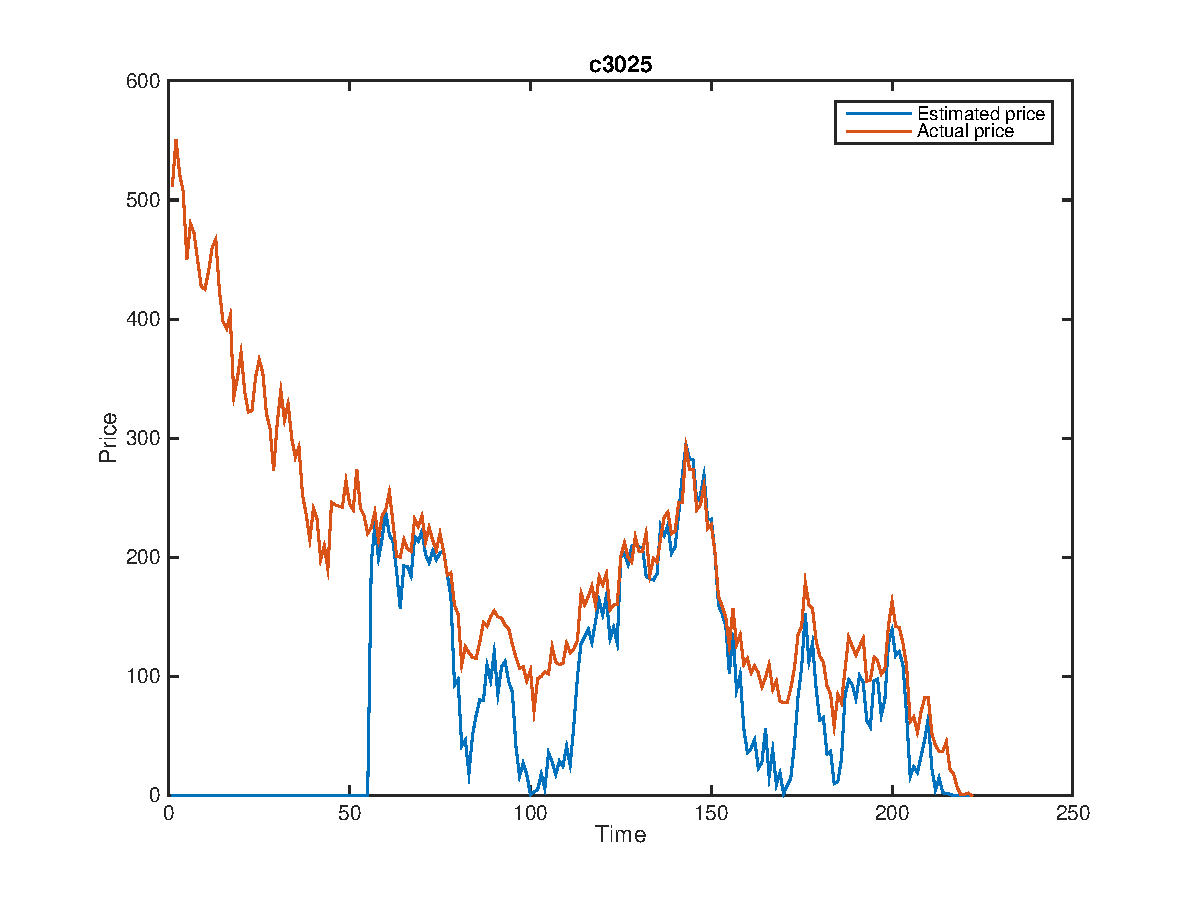
\includegraphics[width=0.32\linewidth]{figures/p2/3.eps}
		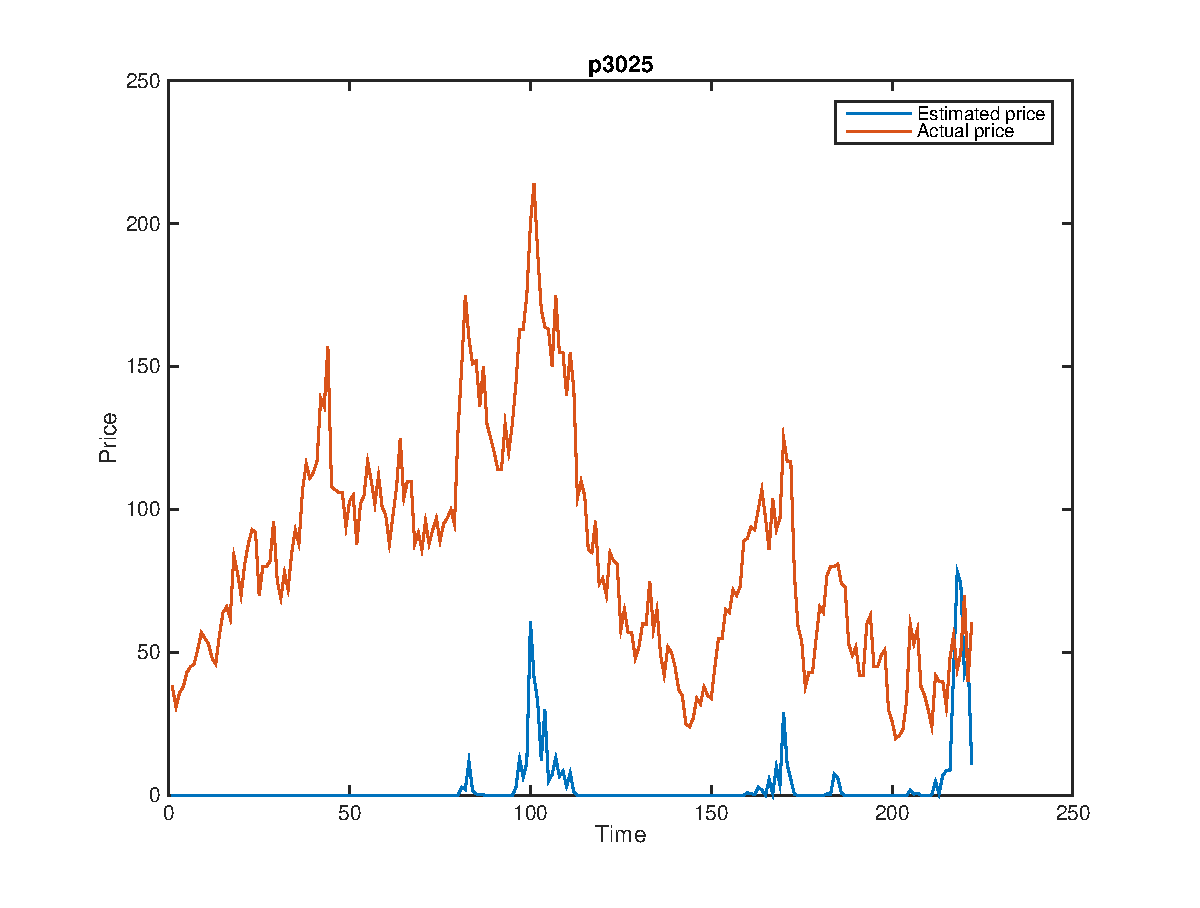
\includegraphics[width=0.32\linewidth]{figures/p2/4.eps}
		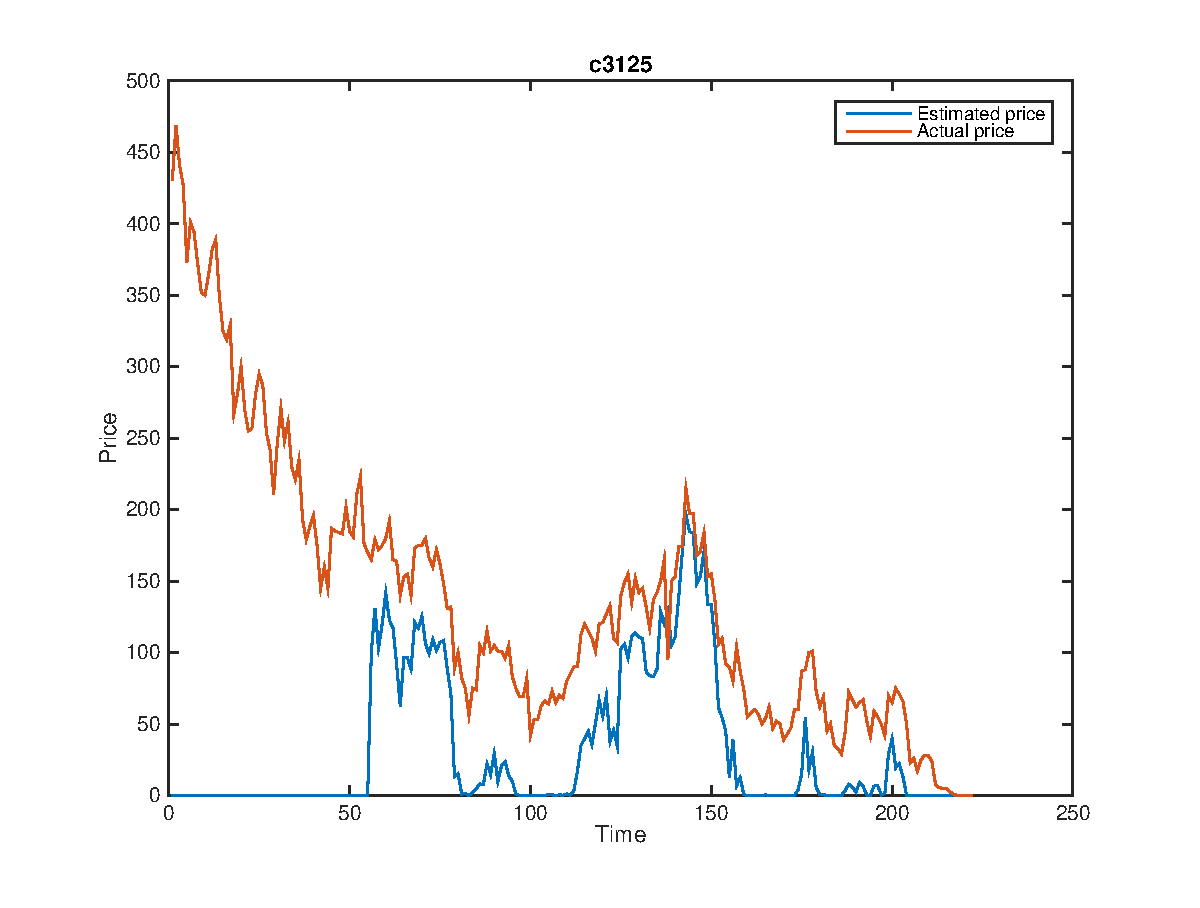
\includegraphics[width=0.32\linewidth]{figures/p2/5.eps}
		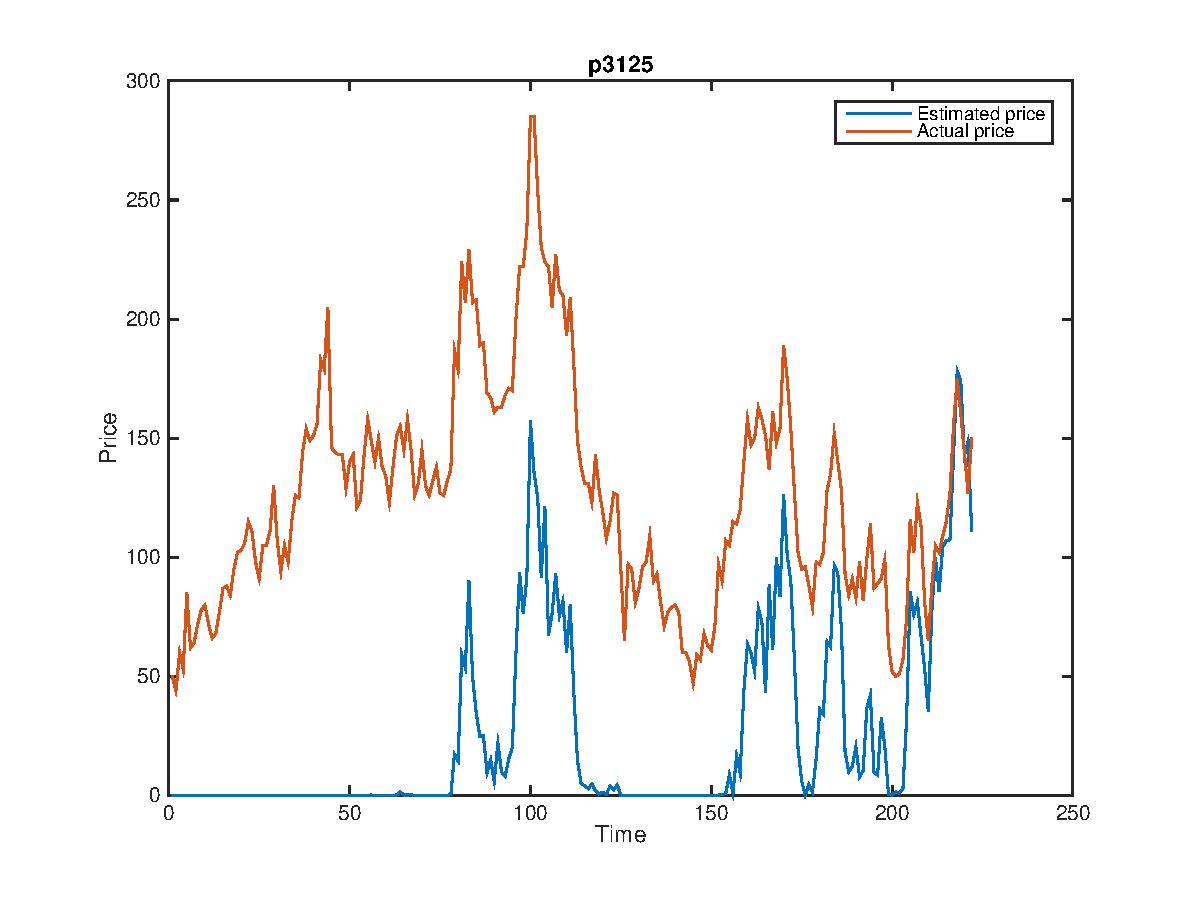
\includegraphics[width=0.32\linewidth]{figures/p2/6.eps}
		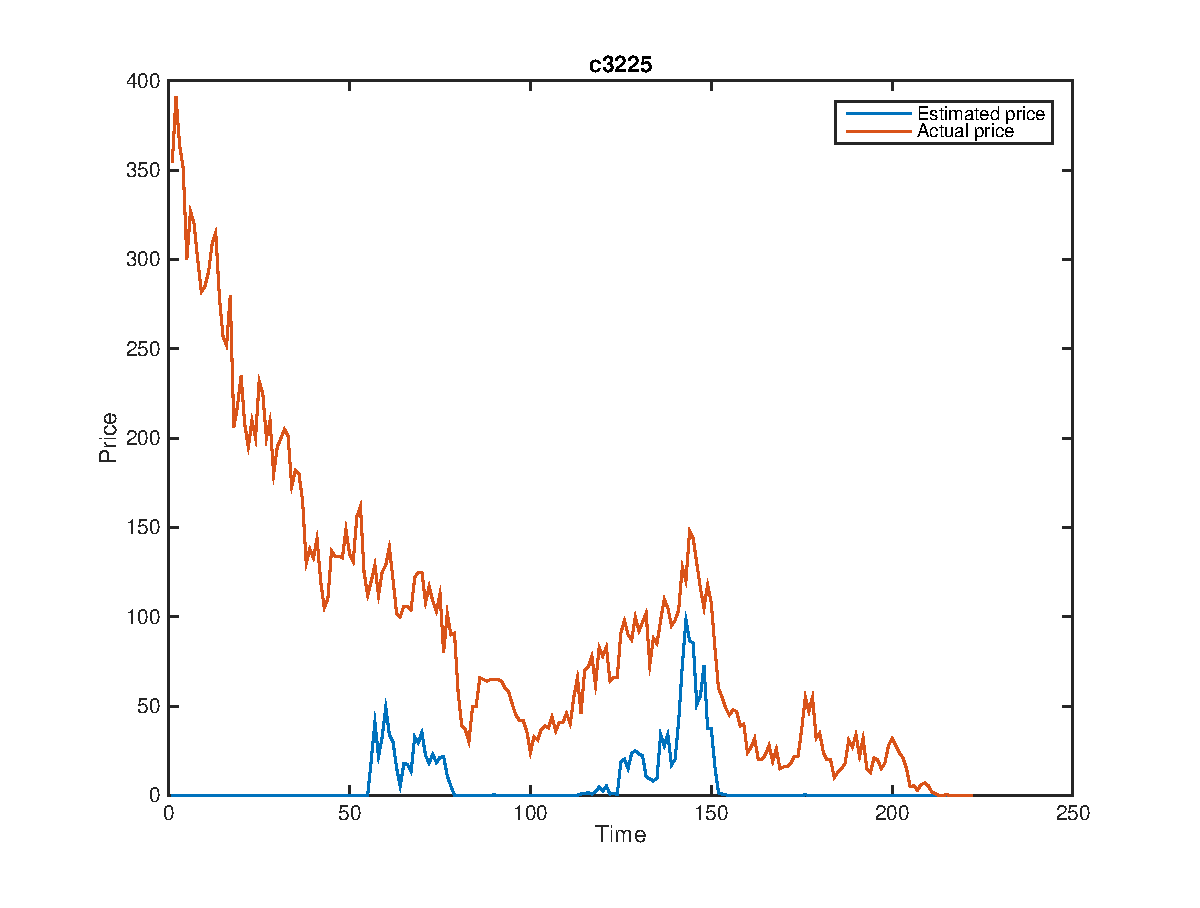
\includegraphics[width=0.32\linewidth]{figures/p2/7.eps}
		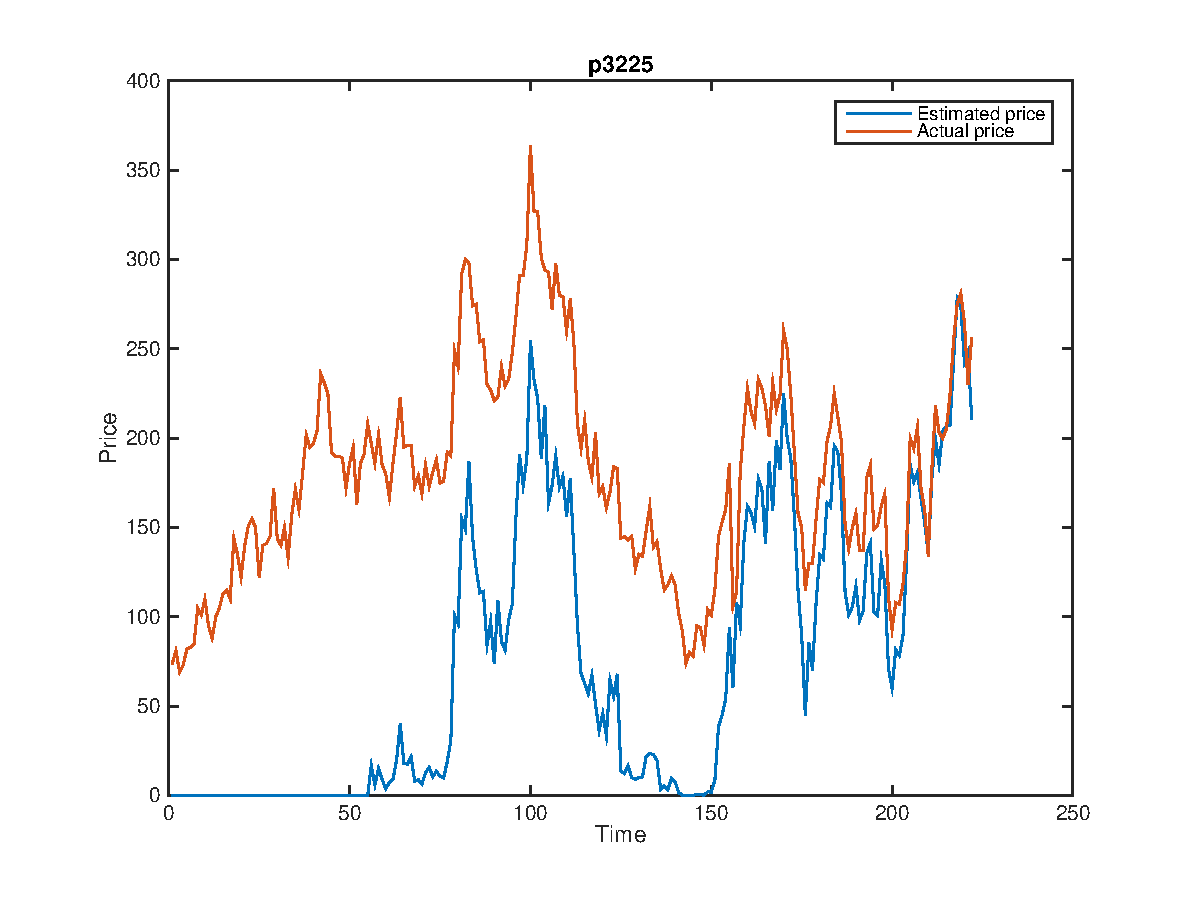
\includegraphics[width=0.32\linewidth]{figures/p2/8.eps}
		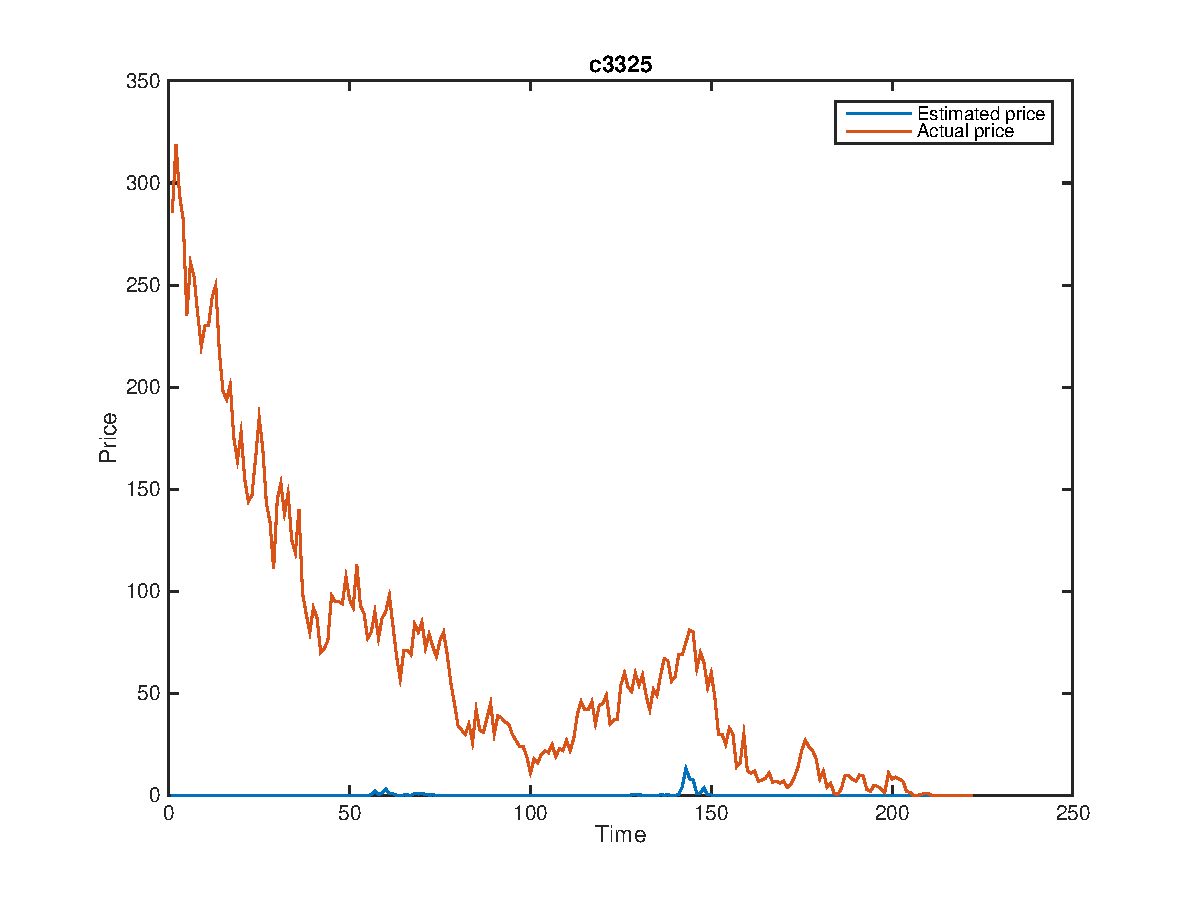
\includegraphics[width=0.32\linewidth]{figures/p2/9.eps}
		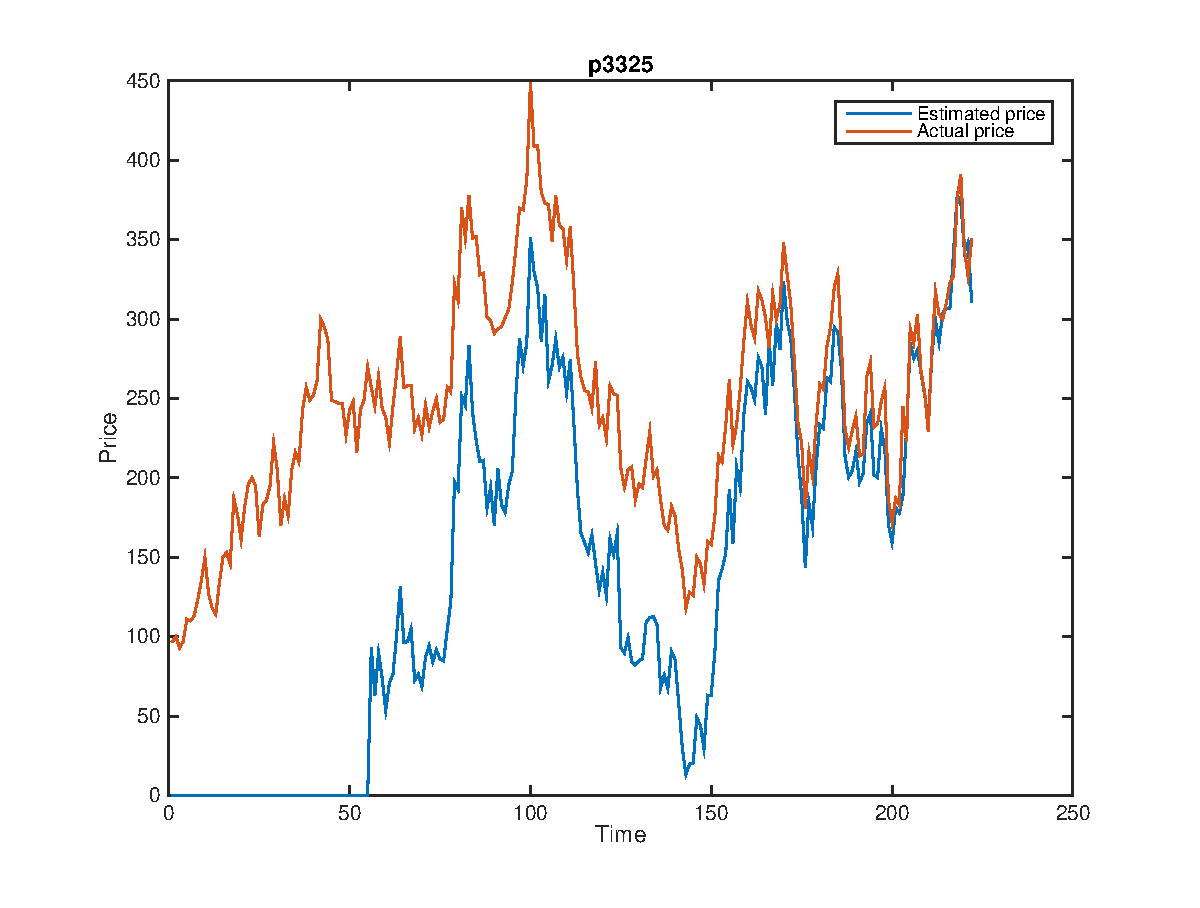
\includegraphics[width=0.32\linewidth]{figures/p2/10.eps}
		\caption{Estimated (from Black-Scholes model) vs. actual option prices for 10 options}
	\end{figure}
	\restoregeometry

	\section{Question 3}

	Figure~\ref{fig:volatilities} shows a plot of implied volatilities (calculated using the \texttt{blsimpv} function) vs estimated volatilities (calculated in the same manner as question 2). The function $y = x$ has been plotted on the same axes for comparison. The estimated volatilities are systematically lower than the implied volatilities.

	\begin{figure}
		\centering
		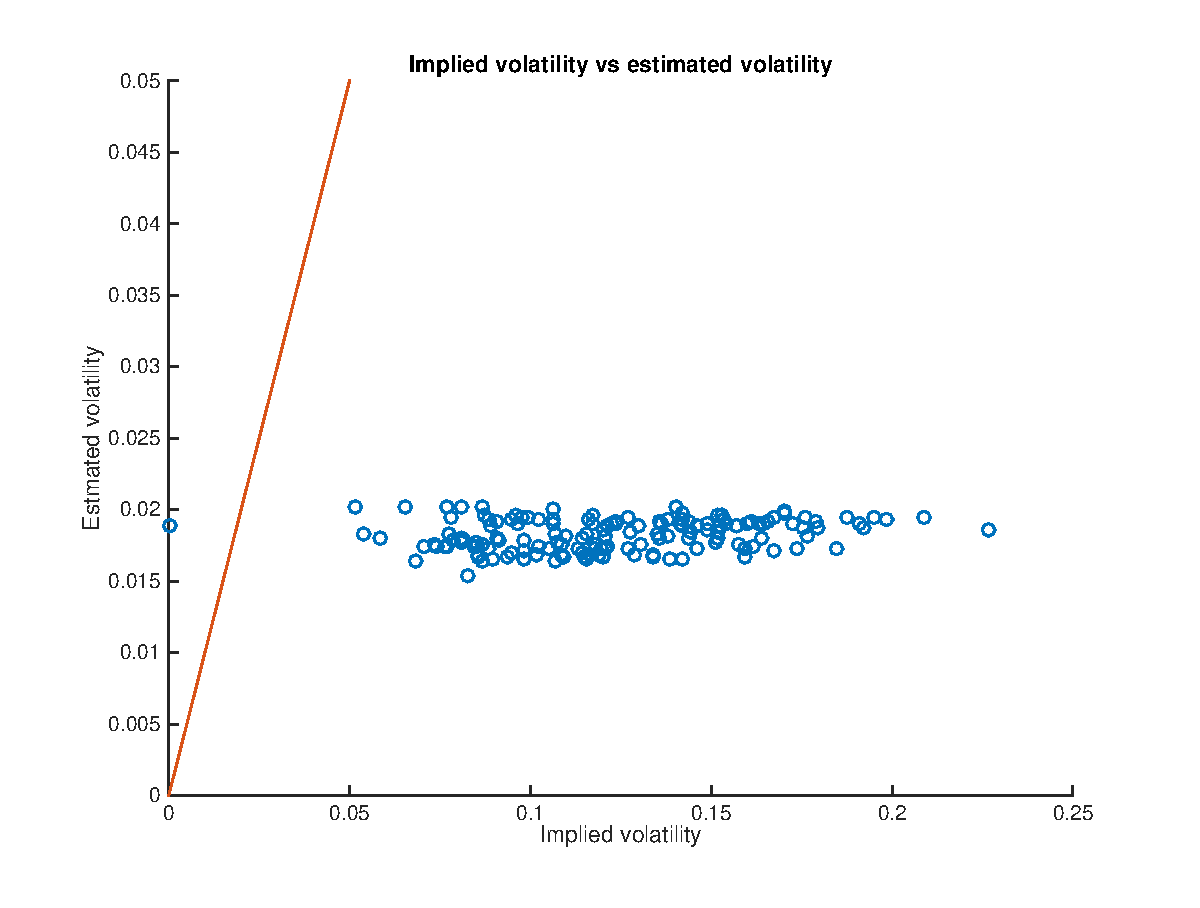
\includegraphics[width=0.5\linewidth]{figures/p3/volatilities.eps}
		\caption{Implied volatility vs estimated volatility}
		\label{fig:volatilities}
	\end{figure}

	The implied volatilities of options at different strike prices were plotted against the strike price, as shown in figure~\ref{fig:t208}. For most days, the implied volatility calculated from the data is \texttt{NaN}. On none of the days do the data appear to produce the ``volatility smile'' mentioned in the question.

	\begin{figure}
		\centering
		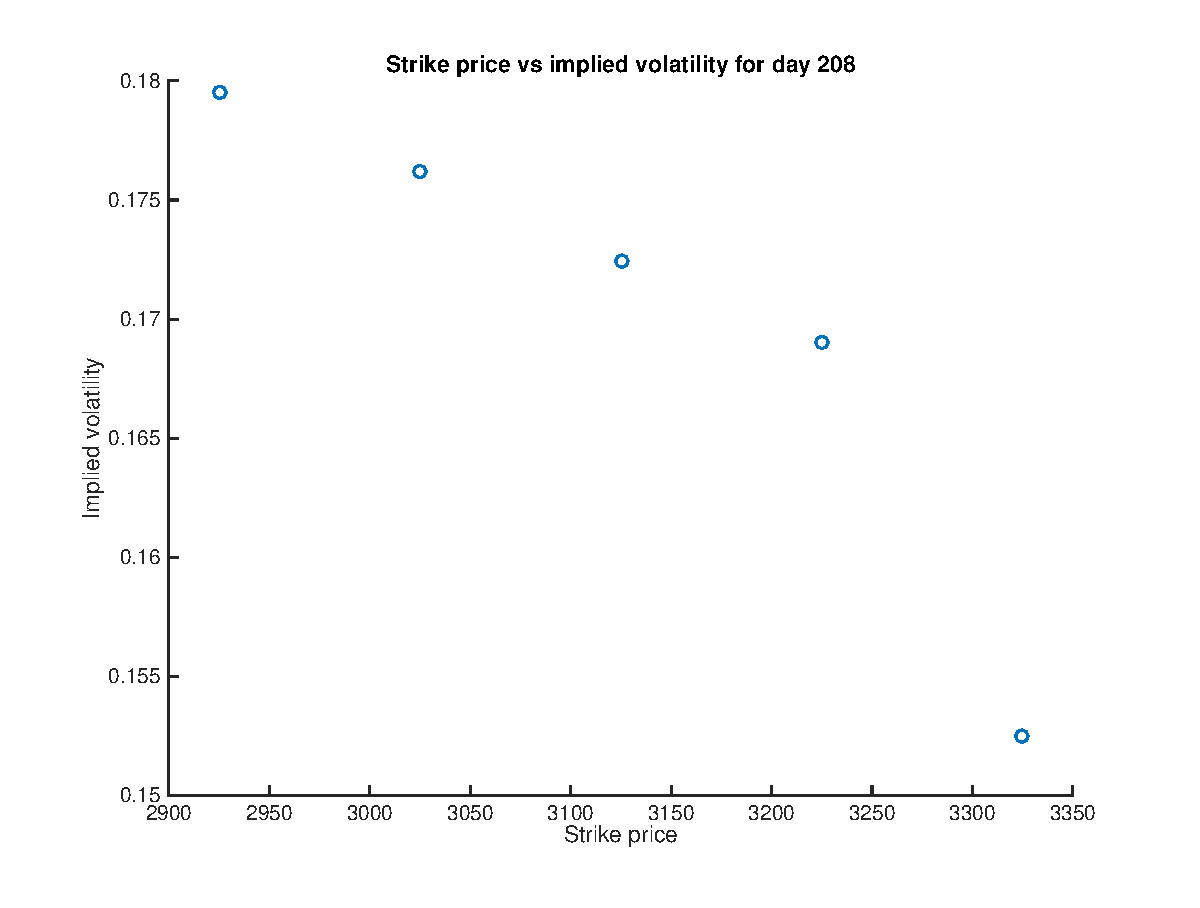
\includegraphics[width=0.5\linewidth]{figures/p3/t208.eps}
		\caption{Strike price vs implied volatility}
		\label{fig:t208}
	\end{figure}

	\section{Question 4}

	American-style options contracts can be exercised at any time between issuance and the date of maturity, whereas European-style contracts may only be exercised at maturity. Because of this, American-style contracts command a higher value as they may be exercised early if it makes financial sense to do so. For example, a trader might wish to exercise a call option if the price of the underlying asset ever rises above the strike price, or exercise a put option if the price ever falls below it.

	\section{Question 5}

	The provided data for the call option with strike price 3025 were used with $t = 75$ to calculate the estimated volatility of the data, and the MATLAB functions \texttt{blsprice} and \texttt{binprice} were used to calculate the option price using the Black-Scholes model and the Binomial Lattice model, respectively. 100 $\delta t$ values in the interval $[0.01, 0.2]$ were used for the Binomial Lattice model, and the absolute differences between the options prices calculated from the two models were plotted against $\delta t$ in figure~\ref{fig:p5}. A $\delta t$ is reduced, the Binomial Lattice model approaches the Black-Scholes model.

	\begin{figure}
		\centering
		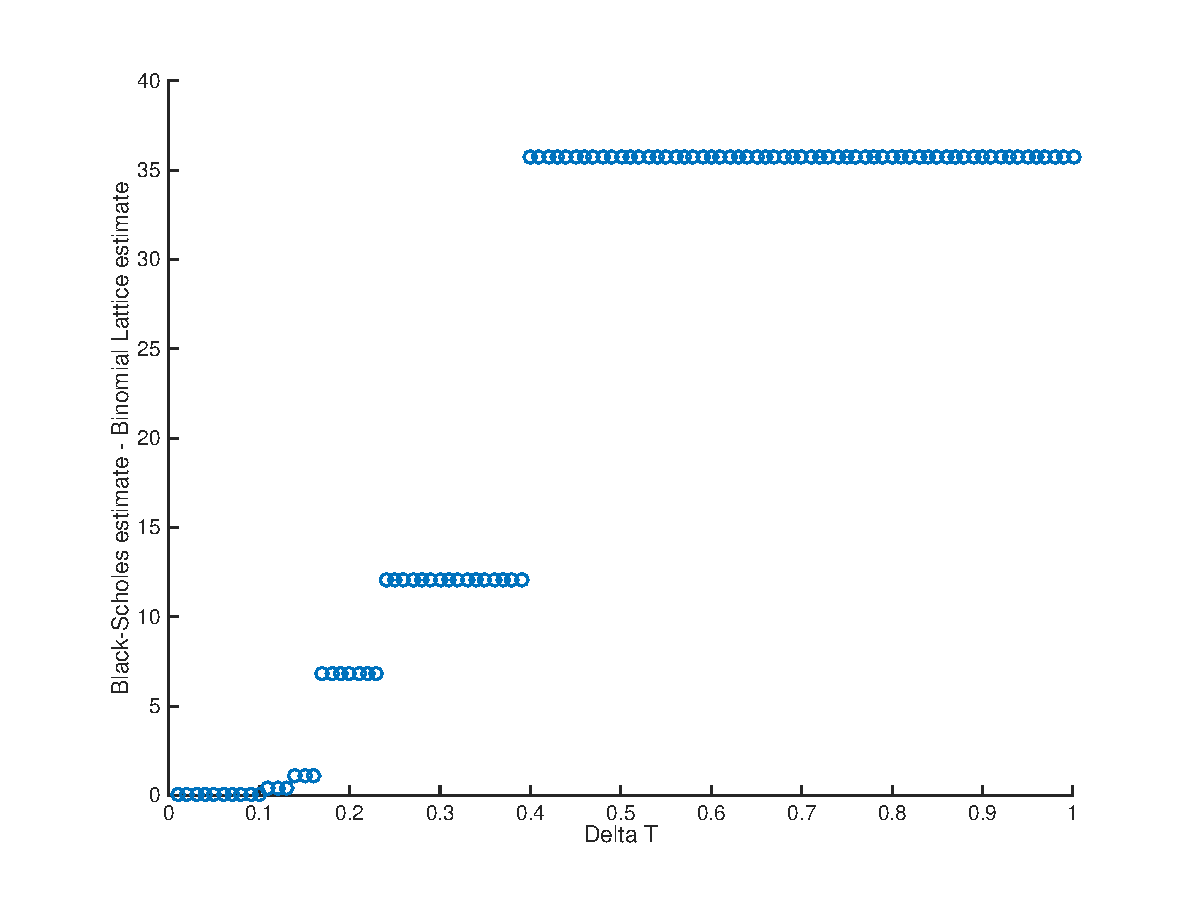
\includegraphics[width=0.5\linewidth]{figures/p5.eps}
		\caption{Absolute difference between Black-Scholes estimate and Binomial estimate as a function of $\delta t$}
		\label{fig:p5}
	\end{figure}

	\section{Question 6}

	The code shown first calculates the profit if the option is held (\texttt{hold}), and the profit if it is exercised now (\texttt{K - SVals(i)}), and takes the maximum of the two to calculate the most profitable strategy at this point in time.

	For pricing a call option, the code would change to the following:

	\begin{verbatim}
	for tau=1:N
	    for i= (tau+1):2:(2*N+1-tau)
	        hold = p_u*PVals(i+1) + p_d*PVals(i-1);
	        PVals(i) = max(hold, SVals(i) - K);
	    end
	end
	\end{verbatim}

	\clearpage
	\appendix

	\section{Code for question 1}

	\begin{verbatim}
		clear;

		x = linspace(30, 55)';
		N = size(x, 1);
		y = zeros(N, 1);

		for n = 1:N
		    if x(n) > 45
		        y(n) = x(n) - 45;
		    elseif x(n) < 40
		        y(n) = 40 - x(n);
		    end
		end

		plot(x, y);
		title('Trader profit as a function of asset price at maturity');
		xlabel('S(T)');
		ylabel('Profit');
	\end{verbatim}

	\section{Code for question 2}

	\begin{verbatim}
		clear;
		load('data.mat');

		for strike_price = 2925:100:3325
		    data1 = dlmread(sprintf('Data/c%d.prn', strike_price));
		    data2 = dlmread(sprintf('Data/p%d.prn', strike_price));
		    stock_prices = data1(:, 3);
		    call_prices = data1(:, 2);
		    put_prices = data2(:, 2);
		    T = size(stock_prices, 1);
		    quarter = floor(T / 4);

		    bls_call_prices = zeros(T, 1);
		    bls_put_prices = zeros(T, 1);
		    for t = (quarter + 1):T
		        window = stock_prices((t-quarter):t);
		        u = tick2ret(window, [], 'Continuous');
		        s = std(u);
		        N = size(window, 1);
		        volatility = s / sqrt(N / 252);
		        [call, put] = blsprice(stock_prices(t), strike_price, 0.06,
		            (T + 1 - t) / 252, volatility);
		        bls_call_prices(t) = call;
		        bls_put_prices(t) = put;
		    end
		    figure;
		    plot(bls_call_prices(1:T));
		    hold on;
		    plot(call_prices(1:T));
		    title(sprintf('c%d', strike_price));
		    legend('Estimated price', 'Actual price');
		    xlabel('Time');
		    ylabel('Price');
		    figure;
		    plot(bls_put_prices(1:T));
		    hold on;
		    plot(put_prices(1:T));
		    title(sprintf('p%d', strike_price));
		    legend('Estimated price', 'Actual price');
		    xlabel('Time');
		    ylabel('Price');
		end
	\end{verbatim}

	\section{Code for question 3}

	\begin{verbatim}
		clear;
		load('data.mat');

		T = size(c3025, 1);
		quarter = round(T/4);

		implied_volatilities = zeros(T, 1);
		calculated_volatilities = zeros(T, 1);

		for t = (quarter + 1):T
		    implied_volatilities(t) = blsimpv(c3025(t, 3), 3025, 0.06,
		        (T + 1 - t) / 252, c3025(t, 2));
		    window = c3025((t-quarter):t, 3);
		    u = tick2ret(window, [], 'Continuous');
		    s = std(u);
		    N = size(window, 1);
		    calculated_volatilities(t) = s / sqrt(N / 252);
		end

		figure;
		scatter(implied_volatilities((quarter + 1):T),
		    calculated_volatilities((quarter + 1):T));
		hold on;
		plot(0:0.05:0.05, 0:0.05:0.05);
		title('Implied volatility vs estimated volatility');
		xlabel('Implied volatility');
		ylabel('Estmated volatility');

		strike_prices = (2925:100:3325)';
		implied_volatilities = zeros(size(strike_prices, 1), 1);

		t = 208;
		for n = 1:size(strike_prices, 1)
		    strike_price = strike_prices(n);
		    data = dlmread(sprintf('Data/c%d.prn', strike_price));
		    T = size(data, 1);
		    implied_volatilities(n) = blsimpv(data(t, 3), strike_price, 0.06,
		        (T + 1 - t) / 252, data(t, 2));
		end

		figure;
		scatter(strike_prices, implied_volatilities);
		title(sprintf('Strike price vs implied volatility for day %d', t));
		xlabel('Strike price');
		ylabel('Implied volatility');
	\end{verbatim}

	\section{Code for question 5}

	\begin{verbatim}
		clear;
		load('data.mat');
		T = size(c3125, 1);
		quarter = round(T / 4);
		t = 75;

		window = c3125((t-quarter):t, 3);
		u = tick2ret(window, [], 'Continuous');
		s = std(u);
		N = size(window, 1);
		volatility = s / sqrt(N / 252);

		diffs = zeros(100, 1);
		deltaTs = linspace(0.01, 0.2, 100);
		for n = 1:100
		    [call, put] = blsprice(c3125(t, 3), 3125, 0.06, (T + 1 - t) / 252,
			    volatility);
		    [AssetPrice, OptionValue] = binprice(c3125(t, 3), 3125, 0.06,
			    (T + 1 - t) / 252, deltaTs(n), volatility, 1);
		    diffs(n) = abs(call - OptionValue(1, 1));
		end
		scatter(deltaTs, diffs);
		xlabel('Delta T');
		ylabel('Black-Scholes estimate - Binomial Lattice estimate');
	\end{verbatim}

\end{document}
